\chapter{Catálogos}

\section{Gaia} \label{muestra:gaia}

Originalmente denominado como GAIA, la misión \textbf{Gaia} fue lanzada por
la \textbf{Agencia Espacial Europea} (\textbf{ESA}) el 19 de Diciembre del 2013, con el
objetivo de generar un mapa tridimensional de la Galaxia.
Esto incluye calcular las propiedades astrométricas y astrofísicas de sus
fuentes observadas con mayor precisión que cualquier otro catálogo publicado
previamente. Para lograr esto se utiliza un satélite espacial, el cual está
denominado como \textit{Gaia}, ubicado en el punto de Lagrange L2 con respecto al
sistema Sol-Tierra. Desde este punto el satélite tiene una vista sin obstrucciones
que le permite observar una cantidad impresionante de objetos, con \textapproxtilde
1,000 millones de fuentes visibles. [\citeyearparen{gaiaMission}] 

\subsection{Data Release 3}

Para facilitar el acceso público a los datos recabados por la misión de \gaia la
ESA ha escogido liberar los datos públicamente conforme los van recibiendo y
procesando. Estos son conocidos como los \textit{Data Releases}. Este trabajo
emplea el \textbf{Data Release 3} (\textbf{GDR3}) el cual está compuesto de las
observaciones hechas por Gaia entre el 25 de Julio del 2014 y el 28 de Mayo del
2017, un periodo de 22 meses en total. GDR3 consiste de información para
\num{1811709771} de fuentes individuales, incluyendo parámetros astrométricos y
datos fotométricos. 

Los datos utilizados en este trabajo fueron obtenidos a través de
\textit{Gaia Archive}\footnote{\url{https://gea.esac.esa.int/archive/}}, una
herramienta libre publicada por la ESA. Esta cuenta con una interfaz de
ADQL\footnote{\url{https://www.ivoa.net/documents/ADQL/20180112/PR-ADQL-2.1-20180112.html}},
un lenguaje estructurado para hacer consultas a las tablas en la base de datos
de Gaia. Aparte de las tablas publicadas por la ESA también se pueden acceder a
tablas publicadas por investigadores como parte de sus trabajos de
investigación, como el de
\citeyearparen{bailer-jones_estimating_distances_gaia_edr3_2021} que reportan
las distancias de las fuentes en el catálogo \textit{eDR3} de Gaia
(\textit{early} Data Release 3, publicado antes del catálogo completo DR3)
corrigiendo por errores sistemáticos en la medición del paralaje de las fuentes.

\subsection{Fotometría}

Compuesto de 2 tubos ópticos que comparten un mismo plano focal, el instrumento
principal de Gaia fue fabricado con el objetivo de escanear el cielo entero,
sistemáticamente obteniendo observaciones de cada objeto que pasa por su campo
de visión, midiendo sus propiedades astrométricas (su paralaje, las componentes
de su posición angular, y las componentes de su movimiento propio) en diferentes
tiempos. Información a detalle de los instrumentos abordo de Gaia se puede
encontrar en la página web de la misma
misión\footnote{\url{https://www.cosmos.esa.int/web/gaia/instruments}}. 

El instrumento fotométrico de Gaia consiste de una matriz de CCDs ubicada en el
plano focal de los tubos ópticos. Estos están divididos en base a su función en
el procesamiento del tránsito de un objeto; un esquema del plano focal se
encuentra en la documentación en línea de
Gaia\footnote{\url{https://www.cosmos.esa.int/web/gaia/focal-plane}}. Tres de
los grupos de CCDs son los de mayor interés en cuanto a las mediciones
fotométricas de Gaia: el \textit{Sky Mapper}, los cuales son responsables de
detectar las fuentes que estén en tránsito del plano focal y de hacer una
primera medición de la magnitud de la fuente en el pasabanda ancha $G$; y los
\textit{fotómetros} \textit{azul} y \textit{rojo}, los cuales toman medidas
espectro-fotométricas de las fuentes en tránsito en las pasabandas $BP$ y $RP$
respectivamente. Las observaciones integradas y procesadas de cada tránsito para
un objeto se pueden extraer por medio de la base de datos \textit{Datalink}
ofrecida como datos complementarios de la base de datos principal de Gaia.
\citetbooksection{gdr3ReleaseDocumentation}{20.7.1} documentan la información
técnica con respecto a los campos de los datos.

\begin{figure}[!ht]
    \centering
    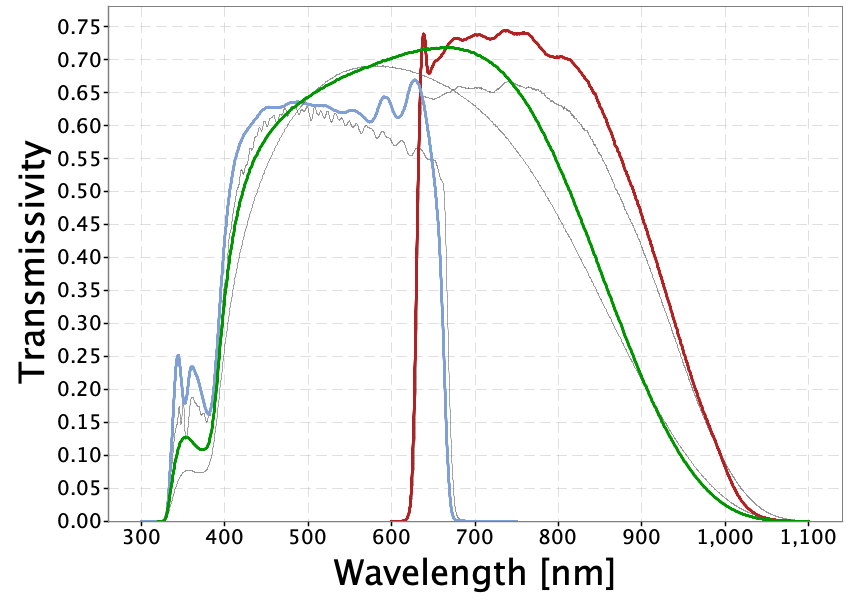
\includegraphics[scale=0.4]{Muestra/Secciones/Figures/Figura Gaia Pasabandas DR3.png}
    \caption{Curvas actualizadas de transmisividad para las pasabandas $G$
    (verde), $G_{BP}$ (azul), y $G_{RP}$ (rojo) para DR3. Las curvas originales
    reportadas antes del lanzamiento de la misión se ven en gris claro en el
    fondo. Figura obtenida de
    \citetbooksection{gdr3ReleaseDocumentation}{5.4.1}.}
    \label{figuraGaiaPasabandasDr3}
\end{figure}

\section{Sloan Digital Sky Survey}

La colección de catálogos \textbf{Sloan Digital Sky
Survey}\footnote{\url{https://www.sdss.org}} (de ahora en adelante será referido
como \textbf{SDSS}) compila varias fuentes de datos astronómicos
en un sitio centralizado, con el objetivo de crear un mapa tridimensional del
Universo con una precisión no vista antes. Estos incluyen imágenes de objetos
astronómicos en varios colores, acompañados de un espectro obtenido como parte
de esta misión. Para finales del siglo XX habían surgido avances
tecnológicos que llegarían a revolucionar la astronomía observacional. De estos,
los de mayor interés ocurrieron con los detectores de estado sólido y en la
capacidad computacional de procesamiento. Partiendo de estos se empezó a
desarrollar la infraestructura necesaria para recabar datos fotométricos y
espectroscópicos.

El instrumento principal utilizado es el telescopio de 2.5m, ubicado en el
observatorio \textit{Apache Point Observatory}, descrito a detalle en
\citeyearparen{sdss2_5mTelescope}. Este telescopio de diseño Ritchey-Chrétien
alimenta dos instrumentos separados; un CCD multi-banda de gran área, y un par
de espectrógrafos alimentados por fibra óptica. Su construcción empezó en 1998,
pero no fue hasta el año 2000 que estuvo operacional.

\subsection{Data Release 9}

SDSS libera datos en colecciones iterativas; es decir cada Data Release (DR)
liberado contiene todas las observaciones que forman parte del DR previo,
agregando los datos recabados durante el periodo de observación para el DR
actual. Cada DR cae bajo una fase de operaciones de SDSS, delimitado tanto por
las fechas de observaciones como por los instrumentos y tipos de datos
disponibles. Para el periodo operacional de GDR2 el catálogo más actual de SDSS 
era el DR9 publicado como parte de SDSS-III
\footnote{\url{https://www.sdss3.org/index.php}}. Esta tercera fase fue marcada
por una gran mejora del equipo espectroscópico, instalando nuevos instrumentos
con los cuales pudieron analizar la dinámica de nuestra Galaxia, al igual que
otras galaxias y planetas gaseosos extra-solares. 

\section{Zwicky Transient Facility}

El censo observacional \textbf{Zwicky Transient Facility} (\textbf{ZTF})
[\citeyearparen{bellm_ztf_overview_performance_first_results_2018}] tiene como
objetivo observar el cielo del hemisferio norte con una cadencia no realizada
antes por su predecesor el \textit{Palomar Transient Factory}. Las observaciones
de ZTF se hacen desde el \textit{Observatorio Palomar}, ubicado en San Diego,
California, haciendo uso del telescopio Schmidt de 48 pulgadas (denominado
\textit{P48}). Gracias a los avances en la tecnología de CCD y la velocidad de
cómputo el sondeo ZTF ofrece una gran mejora en el procesamiento de datos que le
permite reducir el \quotes{tiempo muerto} entre exposiciones consecutivas,
aumentando la resolución temporal de observación de fenómenos transitorios y de
objetos variables. Observaciones de ZTF consisten de tres filtros únicos: 
\textit{ZTF-g}, \textit{ZTF-r}, y \textit{ZTF-i}, cuyas curvas de
transmisividad se pueden ver en la \reffigure{figuraZTFPasabandas}. La
fotometría se calibra con cada imagen utilizando estrellas del
catálogo de \textit{Pan-STARRS 1} para cada cuadrante, asegurando que se tenga
un índice de color correcto. Tanto las imágenes tomadas para cada exposición
como las mediciones de la fotometría reducida están disponibles en Data Releases
en el registro de \textit{Infrared Science Archive} (\textit{IRSA}) en
línea\footnote{\url{http://irsa.ipac.caltech.edu/Missions/ztf.html}}. Este
trabajo de maestría hizo uso del Data Release 20 (DR20), el cual consiste de
observaciones hechas desde Marzo del 2018 hasta Septiembre 2020. Para más
detalles técnicos del procesamiento y la distribución de datos se hace
referencia a \citeyearparen{masci_ztf_data_processing_products_archive_2018}.

\begin{figure}[!ht]
    \centering
    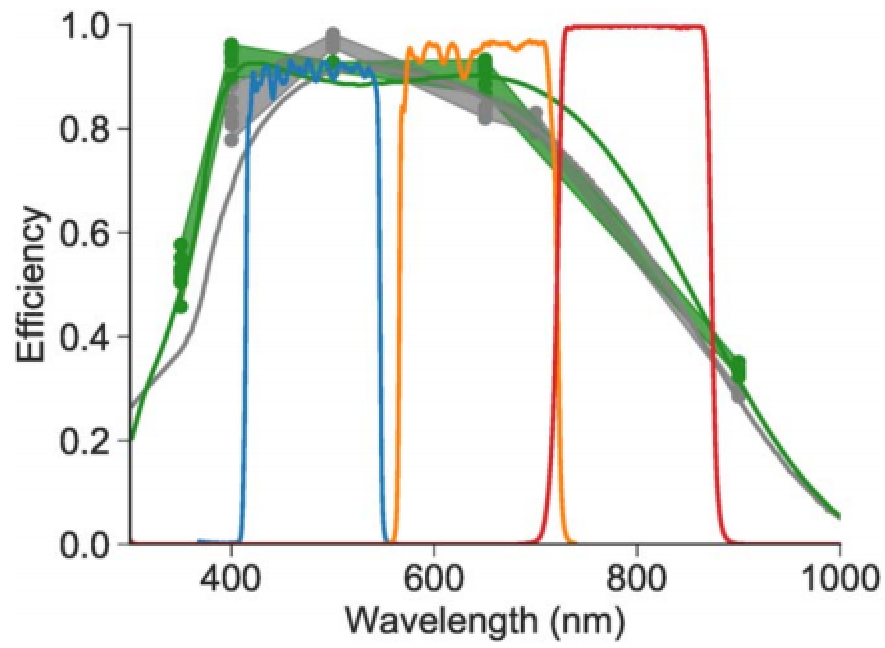
\includegraphics[scale=0.5]{Muestra/Secciones/Figures/Figura ZTF Pasabandas.png}
    \caption{Gráfica de transmisividad para los filtros \textit{ZTF-g},
    \textit{ZTF-r}, y \textit{ZTF-i}, dados por las curvas azul, naranja, y roja
    respectivamente. El campo focal del telescopio P48 está compuesto de un
    mosaico de CCDs que cubren el campo visual entero del telescopio, cubiertos
    por capas anti-reflectantes. Las curvas del fondo representan el modelo de
    la eficiencia cuántica de las CCDs cubiertos por una o dos capas
    anti-reflectantes en gris o verde, respectivamente. Figura obtenida de
    \citeyearparen{bellm_ztf_overview_performance_first_results_2018}.}
    \label{figuraZTFPasabandas}
\end{figure}